\section{Markovian Drone}

\subsection{Optimal Value Heatmap Plot}

\begin{figure}[H]
\centering
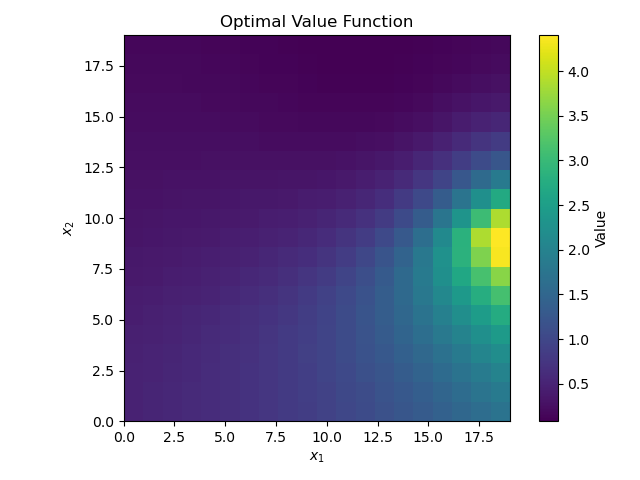
\includegraphics[width=0.5\textwidth]{figures/optimal_value_heatmap.png}
\caption{Optimal Value Heatmap Plot}
\end{figure}

\subsection{Optimal Policy Heatmap Plot}
As seen in Fig. \ref{fig:opt_policy}, the simulated drone is following actions depending on the ego-state, denoted by the heatmap.
Sometimes the policy is overriden by the storm, that is the reason why the drone is taking sometimes different actions than those of the policy.
Also, the simulation runs for 100 steps, so even after reaching the goal, the drone may circle around it. 

\begin{figure}[H]
\centering
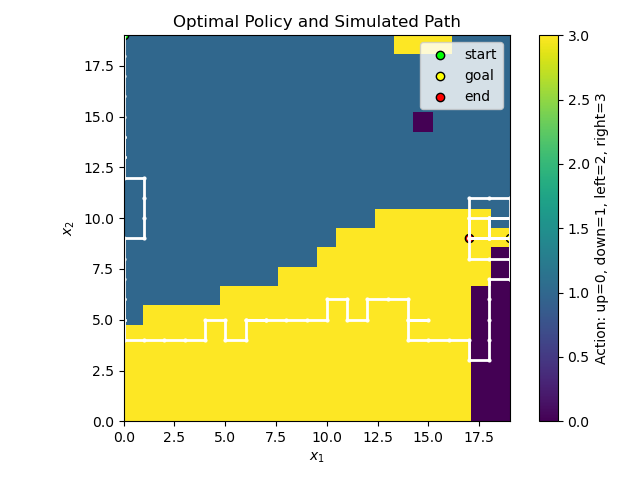
\includegraphics[width=0.5\textwidth]{figures/policy_heatmap_path.png}
\caption{Optimal Policy Heatmap Plot}
\label{fig:opt_policy}
\end{figure}

\subsection{Code}
Code in \hyperref[markovian_drone]{Appendix}.
